\documentclass[a5paper, 10pt]{article}

% Текст
\usepackage[utf8]{inputenc} % UTF-8 кодировка
\usepackage[russian]{babel} % Русский язык
\usepackage{indentfirst} % красная строка в первом параграфе в главе
% Отображение страниц
\usepackage{geometry} % размеры листа и отступов
\usepackage{listings}
\usepackage{color}

\geometry{
	left=12mm,
	top=25mm,
	right=15mm,
	bottom=17mm,
	marginparsep=0mm,
	marginparwidth=0mm,
	headheight=10mm,
	headsep=7mm,
	nofoot}
\usepackage{afterpage,fancyhdr} % настройка колонтитулов
\pagestyle{fancy}
\fancypagestyle{style}{ % создание нового стиля style
	\fancyhf{} % очистка колонтитулов
	\fancyhead[LO, RE]{Лабораторная работа № 4 } % название документа наверху
	\fancyhead[RO, LE]{Задачи 1401, 1604, 1726} % название section наверху
	\fancyfoot[RO, LE]{\thepage} % номер страницы справа внизу на нечетных и слева внизу на четных
	\renewcommand{\headrulewidth}{0.25pt} % толщина линии сверху
	\renewcommand{\footrulewidth}{0pt} % толцина линии снизу
}
\fancypagestyle{plain}{ % создание нового стиля plain -- полностью пустого
	\fancyhf{}
	\renewcommand{\headrulewidth}{0pt}
}
\fancypagestyle{title}{ % создание нового стиля title -- для титульной страницы
	\fancyhf{}
	\fancyhead[C]{{\footnotesize
			Министерство образования и науки Российской Федерации\\
			Федеральное государственное автономное образовательное учреждение высшего образования
	}}
	\fancyfoot[C]{{\large 
			Санкт-Петербург, 2024
	}}
	\renewcommand{\headrulewidth}{0pt}
}

% Математика
\usepackage{amsmath, amsfonts, amssymb, amsthm} % Набор пакетов для математических текстов
%\usepackage{dmvnbase} % мехматовский пакет latex-сокращений
\usepackage{cancel} % зачеркивание для сокращений
% Рисунки и фигуры
\usepackage[pdftex]{graphicx} % вставка рисунков
\usepackage{wrapfig, subcaption} % вставка фигур, обтекая текст
\usepackage{caption} % для настройки подписей
\captionsetup{figurewithin=none,labelsep=period, font={small,it}} % настройка подписей к рисункам
% Рисование
\usepackage{tikz} % рисование
\usepackage{circuitikz}
\usepackage{pgfplots} % графики
% Таблицы
\usepackage{multirow} % объединение строк
\usepackage{multicol} % объединение столбцов
% Остальное
\usepackage[unicode, pdftex]{hyperref} % гиперссылки
\usepackage{enumitem} % нормальное оформление списков
\setlist{itemsep=0.15cm,topsep=0.15cm,parsep=1pt} % настройки списков
% Теоремы, леммы, определения...
\theoremstyle{definition}
\newtheorem{Def}{Определение}
\newtheorem*{Axiom}{Аксиома}
\theoremstyle{plain}
\newtheorem{Th}{Теорема}
\newtheorem{Lem}{Лемма}
\newtheorem{Cor}{Следствие}
\newtheorem{Ex}{Пример}
\theoremstyle{remark}
\newtheorem*{Note}{Замечание}
\newtheorem*{Solution}{Решение}
\newtheorem*{Proof}{Доказательство}
% Свои команды
\newcommand{\comb}[1]{\left[\hspace{-4pt}\begin{array}{l}#1\end{array}\right.\hspace{-5pt} } % совокупность уравнений
% Титульный лист
\usepackage{csvsimple-l3}
\newcommand*{\titlePage}{
	\thispagestyle{title}
	\begingroup
	\begin{center}
		%		{\footnotesize
			%			Министерство образования и науки Российской Федерации\\
			%			Федеральное государственное автономное образовательное учреждение высшего образования
			%		}
		%		
		\vspace*{6ex}
		
		{\small
			САНКТ-ПЕТЕРБУРГСКИЙ НАЦИОНАЛЬНЫЙ ИССЛЕДОВАТЕЛЬСКИЙ УНИВЕРСИТЕТ ИТМО	
		}
		
		\vspace*{2ex}
		
		{\normalsize
			Факультет систем управления и робототехники
		}
		
		\vspace*{15ex}
		
		{\Large \bfseries 
			Лабораторная работа № 4
		}
\vspace*{2ex}
	{\Large \bfseries 
			
"Задачи 1401, 1604, 1726"
		}
\vspace*{2ex}
		
		{\normalsize
			по дисциплине Алгоритмы и структуры данных
		}

	\end{center}
	\vspace*{20ex}
	\begin{flushright}
		{\large 
			\underline{Выполнила}: студентка гр. \textbf{R3238}\\
                             поток \textbf{2.1}\\
			\begin{flushright}
				\textbf{Нечаева А. А.}\\
			\end{flushright}
		}
		
		\vspace*{5ex}
		
		{\large 
			\underline{Преподаватель}: \textit{Тропченко Андрей Александрович}
		}
	\end{flushright}	
	\newpage
	\setcounter{page}{1}
	\endgroup}

\begin{document}
	\titlePage
	\pagestyle{style}

\lstset{ %
language=C,                 % выбор языка для подсветки (здесь это С)
basicstyle=\small\sffamily, % размер и начертание шрифта для подсветки кода
numbers=left,               % где поставить нумерацию строк (слева\справа)
numberstyle=\tiny,           % размер шрифта для номеров строк
stepnumber=1,                   % размер шага между двумя номерами строк
numbersep=5pt,                % как далеко отстоят номера строк от подсвечиваемого кода
backgroundcolor=\color{white}, % цвет фона подсветки - используем \usepackage{color}
showspaces=false,            % показывать или нет пробелы специальными отступами
showstringspaces=false,      % показывать или нет пробелы в строках
showtabs=false,             % показывать или нет табуляцию в строках
frame=single,              % рисовать рамку вокруг кода
tabsize=2,                 % размер табуляции по умолчанию равен 2 пробелам
captionpos=t,              % позиция заголовка вверху [t] или внизу [b] 
breaklines=true,           % автоматически переносить строки (да\нет)
breakatwhitespace=false, % переносить строки только если есть пробел
escapeinside={\%*}{*)}   % если нужно добавить комментарии в коде
}



\newpage
\section{Цель}
Разработать и реализовать алгоритмы для решения задач 1401, 1604 и 1726.


\section{Задача 1401}

\begin{figure}[h]
\center{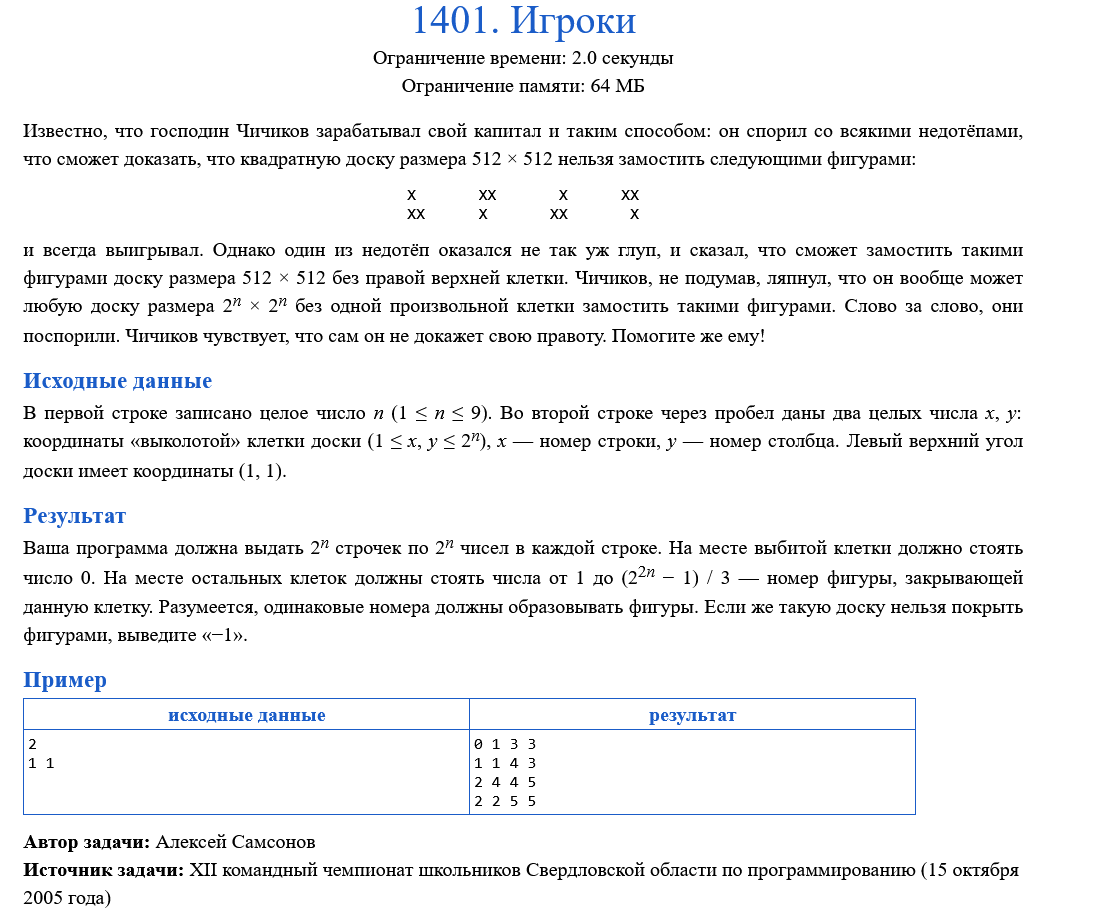
\includegraphics[width=0.9\linewidth]{pic/task_1401.png}}
\caption{Условие задачи 1401.}
\end{figure}

\subsection{Краткое описание алгоритма}
\textbf{1. Входные данные:} в первой строке записано целое число $n\,\, (1 \leq n \leq 9)$. Во второй строке через пробел даны два целых числа $x, \, y$: координаты "выколотой" клетки доски $( 1 \leq x, \, y \leq 2^n )$, $x$ -- номер строки, $y$ -- номер столбца. Левый верхний угол доски имеет координаты $(1, \, 1)$.\\
\textbf{2.} Основу алгоритма составляет \textbf{рекурсия}. Нетрудно заметить, что квадрат 2 на 2 имеет можно замостить требуемым образом. \\
\textbf{3.} По методу математической индукции докажем, что можно замостить требуемым образом квадрат размером $2^n$ на $2^n$. Пусть для квадратов $2^n$ на $2^n$ задача решена, тогда покажем, что для квадрата  $2^{n + 1}$ на $2^{n + 1}$ решение также существует. \\
\textbf{4.} Разобьем большой квадрат на 4 квадрата размера $2^n$ на $2^n$, в одном из них содержится выколотая клетка, значит, мы можем его замостить, по предположению индукции. Вырежем треугольник из центра большого исходного квадрата и получим 3 малых квадрата, у каждого из которых 1 выколотая клетка, опять же по предположению индукции задача для них решена, значит, решена и задача для всего большого квадрата. \\
\textbf{5. Выходные данные:}  программа должна выдать $2^n$ строчек по $2^n$ чисел в каждой строке. На месте выбитой клетки должно стоять число $0$. На месте остальных клеток должны стоять числа от $1$ до $(2^{2n} - 1) / 3$ -- номер фигуры, закрывающей данную клетку. Разумеется, одинаковые номера должны образовывать фигуры. Если же такую доску нельзя покрыть фигурами, вывести $-1$.

\subsection{Листинг}

\begin{center}
\begin{lstlisting}[label=some-code,caption={Исходный код для 1401}]
#include <iostream>
#include <cmath>


int result_points[512][512];
int current_number = 3;


void creator(int n, int x, int y,  int empty_x, int empty_y) {
    // base square
    if (n == 2) {
        for (int i = 0; i < n; ++i) {
            for (int j = 0; j < n; ++j) {
                if (x + i != empty_x || y + j != empty_y) {
                    result_points[x + i][y + j] = current_number / 3;
                    ++current_number;
                }
            }
        }
        return;
    }
    // work with middle triangle
    for (int i = 0; i < 2; ++i) {
        for (int j = 0; j < 2; ++j) {
            int x_1 = x + i * n / 2;
            int x_2 = x + i * n / 2 + n / 2;
            int y_1 = y + j * n / 2;
            int y_2 =  y + j * n / 2 + n / 2;
            
            if (x_1 > empty_x || x_2 <= empty_x ||
            y_1 > empty_y || y_2 <= empty_y) {
                result_points[x + n / 2 - 1 + i][y + n / 2 - 1 + j] = current_number / 3;
                ++current_number;
            }
        }
    }

    for (int i = 0; i < 2; ++i) {
        for (int j = 0; j < 2; ++j) {
            int x_1 = x + i * n / 2;
            int x_2 = x + i * n / 2 + n / 2;
            int y_1 = y + j * n / 2;
            int y_2 = y + j * n / 2 + n / 2;

            // parts with empty point and without
            x_1 <= empty_x && x_2 > empty_x &&
            y_1 <= empty_y && y_2 > empty_y ?
            creator(n / 2, x_1, y_1, empty_x, empty_y) :
            creator(n / 2, x_1, y_1, x + n / 2 - 1 + i, y + n / 2 - 1 + j);
        }
    }
}

int main() {
    int n, empty_x, empty_y;
    std::cin >> n >> empty_x >> empty_y;
    n = pow(2, n);

    creator(n, 0, 0, empty_x - 1, empty_y - 1);

    for (int i = 0; i < n; ++i) {
        for (int j = 0; j < n; ++j) {
            std::cout << result_points[i][j] << " ";
        }
        std::cout << std::endl;
    }
    return 0;
}

\end{lstlisting}
\end{center}

\subsection{Результат}
\begin{figure}[h]
\center{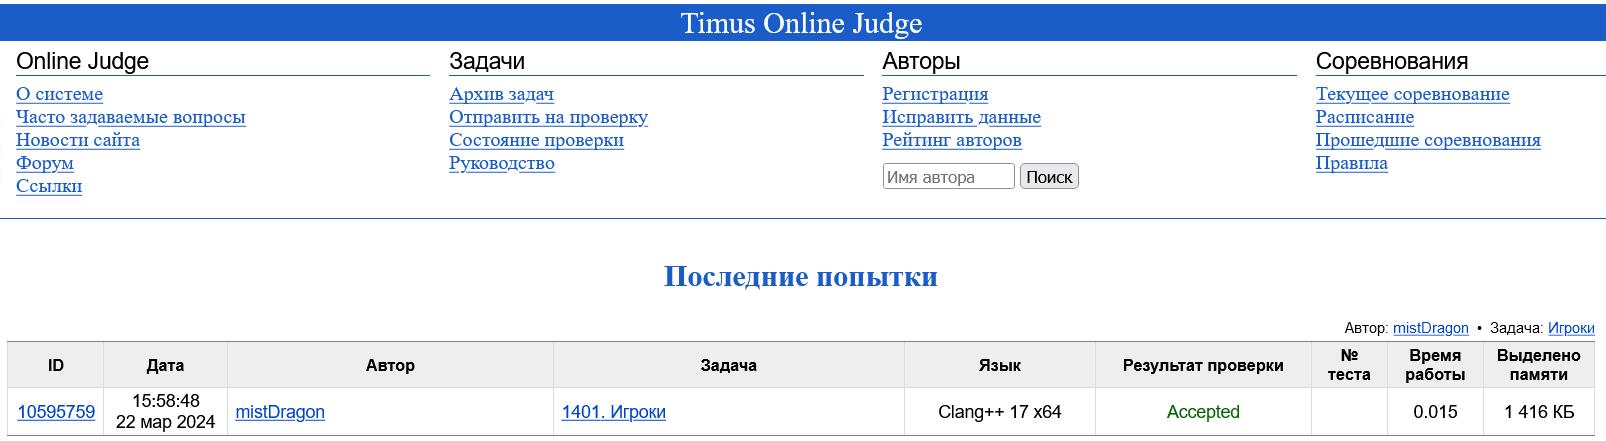
\includegraphics[width=0.9\linewidth]{pic/screen_1401.png}}
\caption{Результат отправки задачи 1401.}
\end{figure}



\newpage

\section{Задача 1604}

\begin{figure}[h]
\center{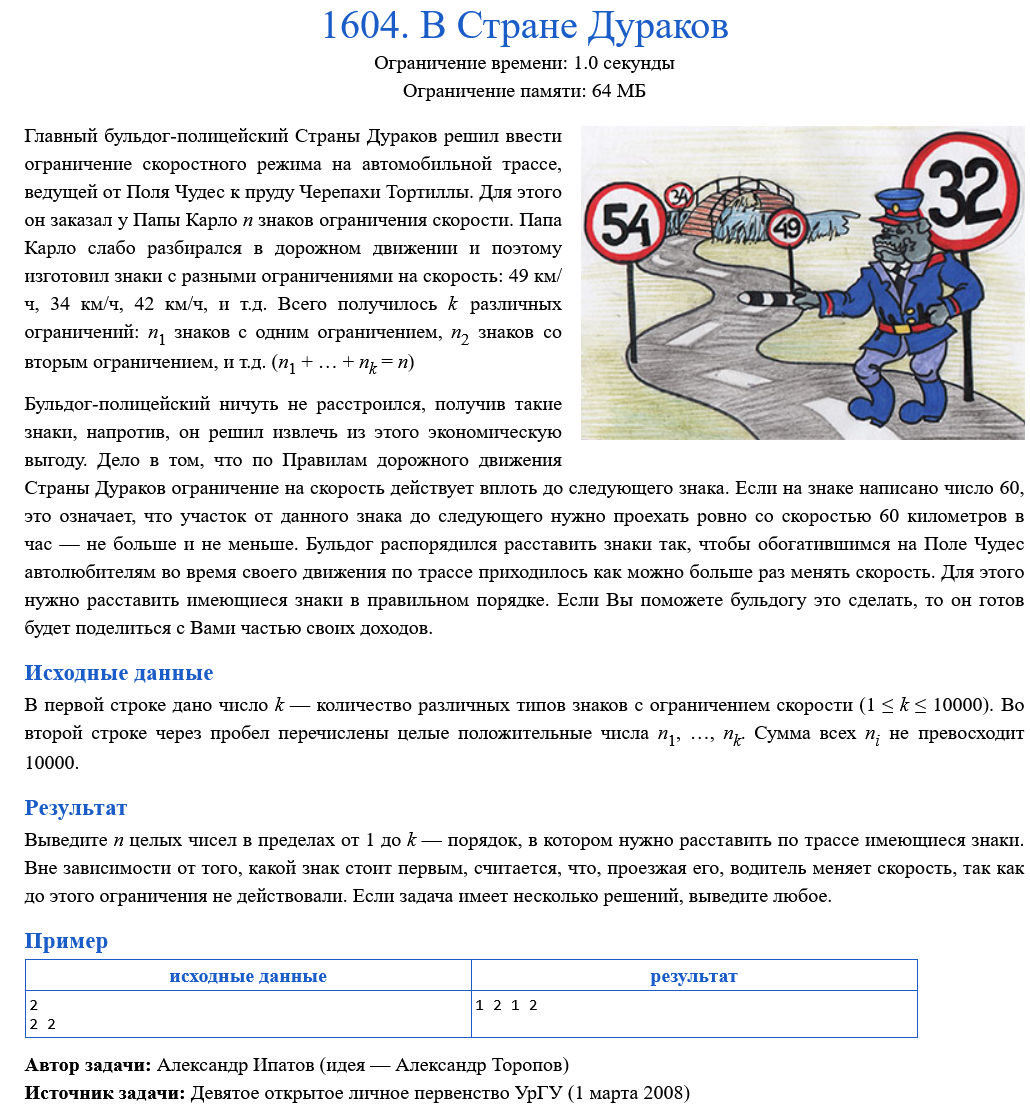
\includegraphics[width=0.9\linewidth]{pic/task_1604.png}}
\caption{Условие задачи 1604.}
\end{figure}

\subsection{Краткое описание алгоритма}
\textbf{1. Входные данные:} в первой строке дано число $k$ -- количество различных типов знаков с ограничением скорости $(1 \leq k \leq 10000)$. Во второй строке через пробел перечислены целые положительные числа $n_1, \ldots , n_k$. Сумма всех $n_i$ не превосходит 10000.\\
\textbf{2.} Сначала применим к исходному массиву знаков сортировку по количеству.\\
\textbf{3.}  Если наибольшее количество знаков больше половины суммарного количества всех знаков, расставим через одного оставшиеся знаки, начиная с первой позиции, так мы добьемся максимального количества смен, на остальные места расставим знаки наибольшего по количеству знака.\\
\textbf{4.} В противном случае расставим по порядку через одного все знаки, таким образом, каждый раз будет происходить смена, потому что количество каждого знака меньше половины от суммарного. \\
\textbf{5.  Выходные данные:} вывести $n$ целых чисел в пределах от $1$ до $k$ -- порядок, в котором нужно расставить по трассе имеющиеся знаки. Вне зависимости от того, какой знак стоит первым, считается, что, проезжая его, водитель меняет скорость, так как до этого ограничения не действовали. Если задача имеет несколько решений, вывести любое.

\subsection{Листинг}

\begin{center}
\begin{lstlisting}[label=some-code,caption={Исходный код для 1604}]
#include <iostream>


std::pair<int, int> signs[10000];

bool compare(std::pair<int, int> s_1, std::pair<int, int> s_2) {
    return s_1.second > s_2.second;
}

//quicksort
void sorter(int left, int right) {
    int i = left;
    int j = right;

    std::pair<char, int> cur = signs[(left + right) / 2];

    while (i <= j) {
        while (compare(signs[i], cur)) {
            ++i;
        }
        while (compare(cur, signs[j])) {
            --j;
        }

        if (i <= j) {
            std::swap(signs[i++], signs[j--]);
        }
    }

    if (i < right) sorter(i, right);

    if (j > left) sorter(left, j);

}

int main() {
    int k;
    std::cin >> k;

    int sum = 0;

    for (int i = 0; i < k; ++i) {
        std::cin >> signs[i].second;
        signs[i].first = i + 1;
        sum += signs[i].second;
    }

    sorter(0, k - 1);
    int res[sum];

    bool check = false;
    if (signs[0].second > (sum + 1) / 2) {
        int i = 1;
        int j = k - 1;

        while (i < sum) {
            res[i] = signs[j].first;
            --signs[j].second;
            signs[j].second == 0 ? --j : j;
            i += 2;

            if (!check && i > sum - 1) {
                check = true;
                i = 0;
            }
        }
    } else {
        int i = 0;
        int j = 0;

        while (i < sum) {
            res[i] = signs[j].first;
            --signs[j].second;
            signs[j].second == 0 ? ++j : j;
            i += 2;

            if (!check && i > sum - 1) {
                check = true;
                i = 1;
            }
        }
    }

    for (int i = 0; i < sum; ++i) {
        std::cout << res[i] << " ";
    }
    return 0;
}
\end{lstlisting}
\end{center}

\subsection{Результат}
\begin{figure}[h]
\center{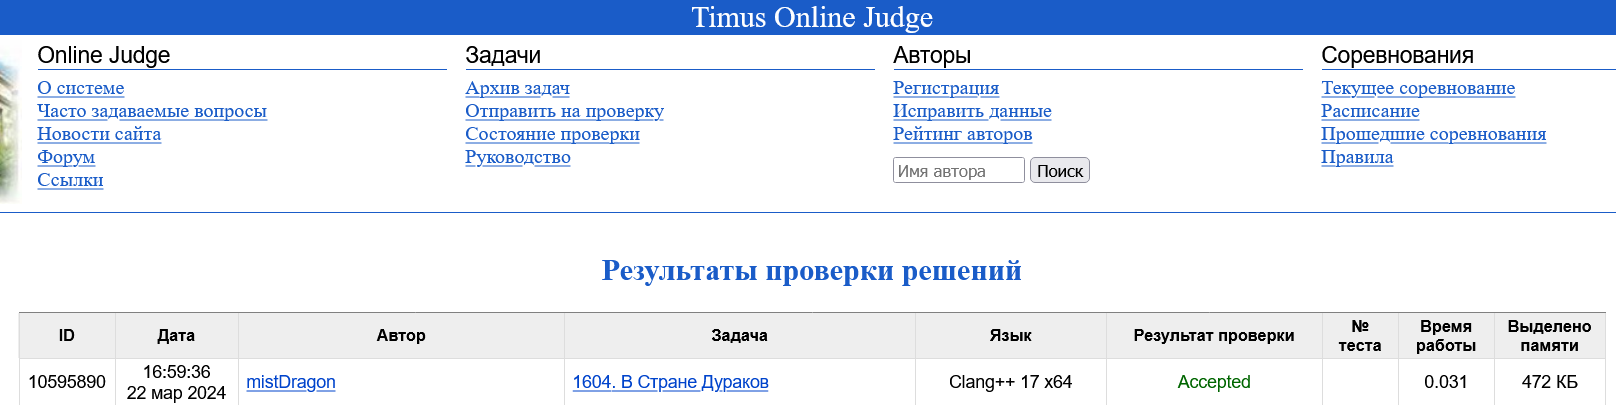
\includegraphics[width=0.9\linewidth]{pic/screen_1604.png}}
\caption{Результат отправки задачи 1604.}
\end{figure}








\newpage


\section{Задача 1726}

\begin{figure}[h]
\center{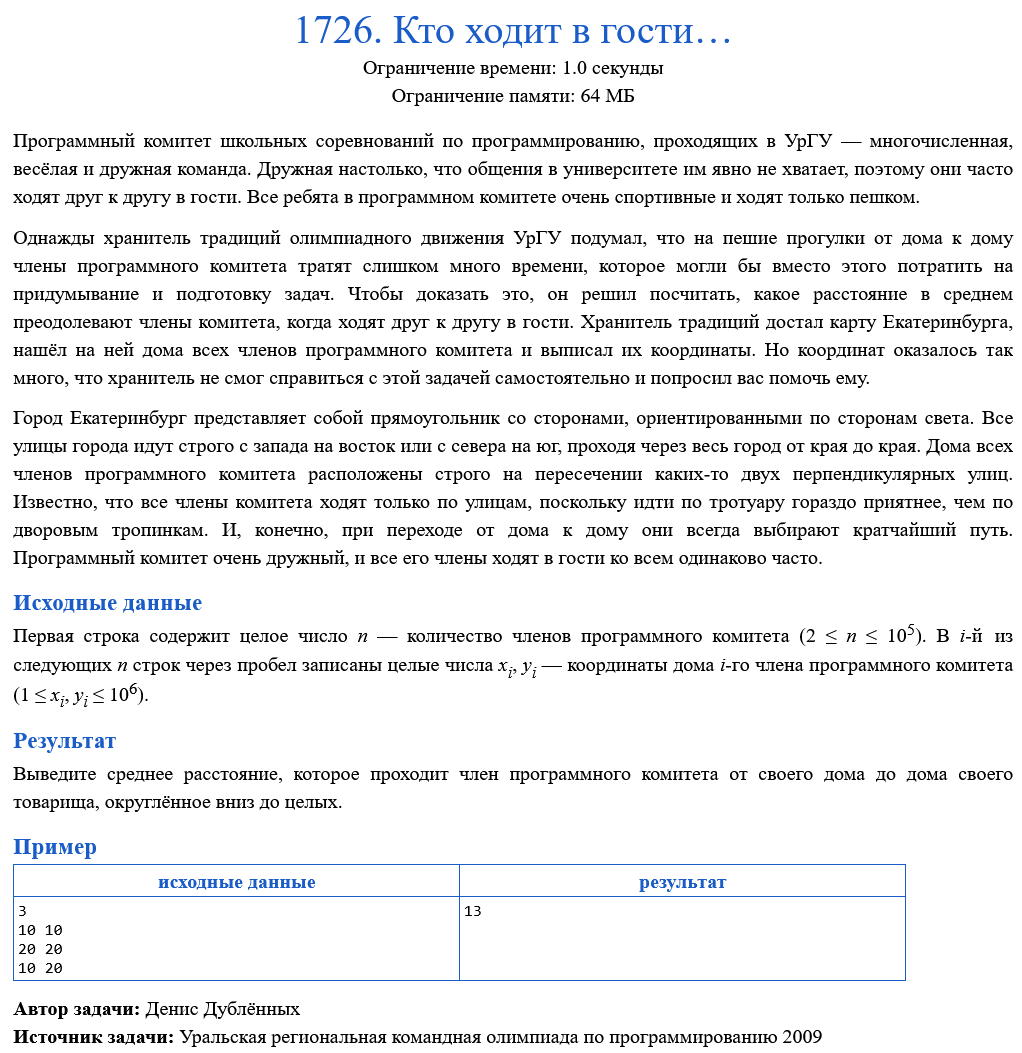
\includegraphics[width=0.9\linewidth]{pic/task_1726.png}}
\caption{Условие задачи 1726.}
\end{figure}

\subsection{Краткое описание алгоритма}
\textbf{1. Входные данные:} \\
\textbf{2.}  \\
\textbf{3.}  \\
\textbf{4.}  \\
\textbf{5.} Выходные данные: 

\subsection{Листинг}

\begin{center}
\begin{lstlisting}[label=some-code,caption={Исходный код для 1726}]
#include <iostream>


\end{lstlisting}
\end{center}

\subsection{Результат}
%\begin{figure}[h]
%\center{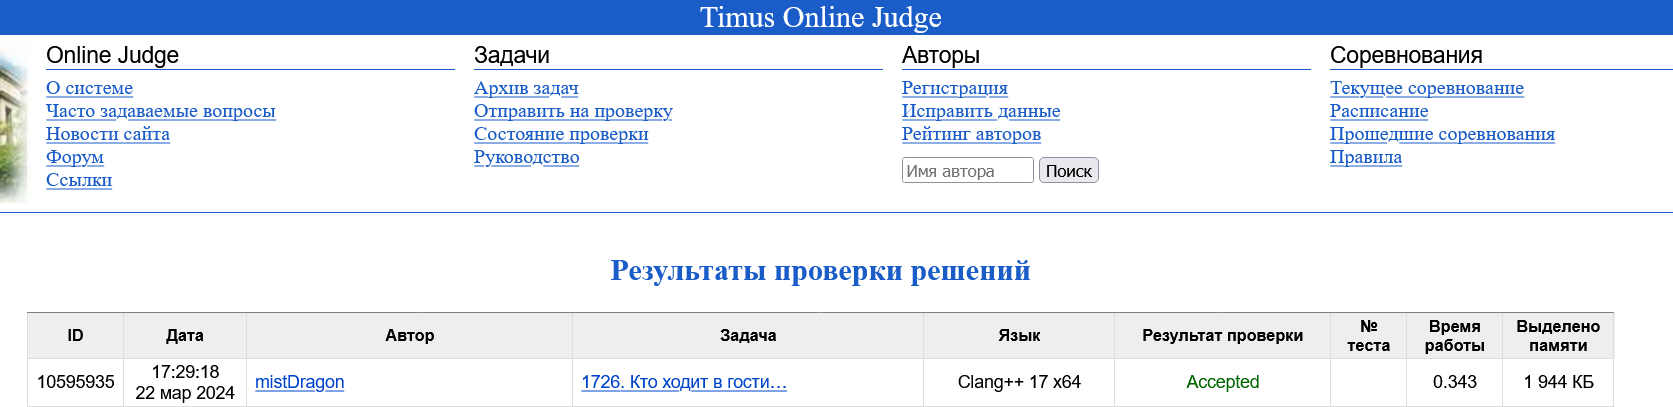
\includegraphics[width=0.9\linewidth]{pic/screen_1726.png}}
%\caption{Результат отправки задачи 1726.}
%\end{figure}



\newpage
\section{Вывод по работе}
В ходе выполнения данной лабораторной работы были реализованы алгоритмы для решения задач $1401$, $1604$ и $1726$. 
\end{document}













